
\documentclass[notheorems,serif]{beamer}

%选用主题
%\usetheme{Rochester}
%\usetheme{default}
%\usetheme{AnnArbor}
%\usetheme{Antibes}
%\usetheme{Bergen}
%\usetheme{Berkeley}
%\usetheme{Berlin}
%\usetheme{Boadilla}
%\usetheme{CambridgeUS}
%\usetheme{Copenhagen}
%\usetheme{Darmstadt}
%\usetheme{Dresden}
%\usetheme{Frankfurt}
%\usetheme{Goettingen}%
%\usetheme{Hannover}
%\usetheme{Ilmenau}
%\usetheme{JuanLesPins}
%\usetheme{Luebeck}
\usetheme{Madrid}
%\usetheme{Malmoe}
%\usetheme{Marburg}
%\usetheme{Montpellier}
%\usetheme{PaloAlto}
%\usetheme{Pittsburgh}
%\usetheme{Rochester}
%\usetheme{Singapore}
%\usetheme{Szeged}
%\usetheme{Warsaw}

% As well as themes, the Beamer class has a number of color themes
% for any slide theme. Uncomment each of these in turn to see how it
% changes the colors of your current slide theme.

%\usecolortheme{albatross}
%\usecolortheme{beaver}
%\usecolortheme{beetle}
%\usecolortheme{crane}
%\usecolortheme{dolphin}
%\usecolortheme{dove}
%\usecolortheme{fly}
%\usecolortheme{lily}
%\usecolortheme{orchid}
%\usecolortheme{rose}
%\usecolortheme{seagull}
%\usecolortheme{seahorse}
%\usecolortheme{whale}
%\usecolortheme{wolverine}

%设置被cover的内容不显示
%\setbeamercovered{transparent}

\useinnertheme{rounded}
\usecolortheme{default}

%调用包
\usepackage[no-math, cm-default]{fontspec}
\usepackage{xltxtra}
\usepackage{xunicode}   
\usepackage{xcolor}
\usepackage{amsmath,amssymb}
\usepackage{xeCJK}
\usepackage{multimedia}
\usepackage{listings}
\usepackage{subfigure}
\usepackage{todonotes}
\presetkeys{todonotes}{inline}{} 
\usepackage{multicol}
\usepackage{changes}




%将系统字体名映射为逻辑字体名称,主要是为了维护的方便  
\newcommand\fnhei{Adobe 黑体 Std}  
\newcommand\fnsong{Adobe 宋体 Std}  
\newcommand\fnkai{Adobe 楷体 Std}  
\newcommand\fnmono{DejaVu Sans Mono}  
\newcommand\fnroman{Times New Roman}  

\renewcommand{\normalsize}{\wuhao}

%%设置常用中文字号,方便调用  
\newcommand{\erhao}{\fontsize{22pt}{\baselineskip}\selectfont}  
\newcommand{\xiaoerhao}{\fontsize{18pt}{\baselineskip}\selectfont}  
\newcommand{\sanhao}{\fontsize{16pt}{\baselineskip}\selectfont}  
\newcommand{\xiaosanhao}{\fontsize{15pt}{\baselineskip}\selectfont}  
\newcommand{\sihao}{\fontsize{14pt}{\baselineskip}\selectfont}  
\newcommand{\xiaosihao}{\fontsize{12pt}{\baselineskip}\selectfont}  
\newcommand{\wuhao}{\fontsize{10.5pt}{\baselineskip}\selectfont}  
\newcommand{\xiaowuhao}{\fontsize{9pt}{\baselineskip}\selectfont}  
\newcommand{\liuhao}{\fontsize{7.5pt}{\baselineskip}\selectfont}  

%\setmainfont{\fnroman}
\setmainfont{\fnkai}
\setCJKmainfont[BoldFont=\fnhei]{\fnkai}  
\setCJKsansfont[BoldFont=\fnhei]{\fnkai}  
\setCJKmonofont{\fnkai}  

%楷体  
%\newfontinstance\KAI{\fnkai}  
%\newcommand{\kai}[1]{{\KAI#1}}  
%黑体  
%\newfontinstance\HEI{\fnhei}  
%\newcommand{\hei}[1]{{\HEI#1}}  
%英文  
%\newfontinstance\ENF{\fnroman}  
%\newcommand{\en}[1]{\,{\ENF#1}\,}

%楷体  
\newfontfamily\KAI {\fnkai}  
\newcommand{\kai}[1]{{\KAI#1}}  
%黑体  
\newfontfamily\HEI{\fnhei}  
\newcommand{\hei}[1]{{\HEI#1}}  
%英文  
\newfontfamily\ENF{\fnroman}  
\newcommand{\en}[1]{\,{\ENF#1}\,}


%连字符
\defaultfontfeatures{Mapping=tex-text}

%中文断行
\XeTeXlinebreaklocale "zh"
\XeTeXlinebreakskip = 0pt plus 1pt minus 0.1pt


%%%% 定理类环境的定义 %%%%
\newtheorem{example}{\hei{例子}} 
\newtheorem{problem}{\hei{问题}}           
\newtheorem{algorithm}{\hei{算法}}
\newtheorem{theorem}{\hei{定理}}
\newtheorem{definition}{\hei{定义}}
\newtheorem{axiom}{\hei{公理}}
\newtheorem{property}{\hei{性质}}
\newtheorem{proposition}{\hei{命题}}
\newtheorem{lemma}{\hei{引理}}
\newtheorem{corollary}{\hei{推论}}
\newtheorem{remark}{\hei{注解}}
\newtheorem{condition}{\hei{条件}}
\newtheorem{conclusion}{\hei{结论}}
\newtheorem{assumption}{\hei{假设}}

%重定义一些环境的名字
\renewcommand{\proofname}{\hei{证明}}
\renewcommand\tablename{\hei{表}}

%---SCRIPT-----------------------------------------------------------------------------------------
\newcommand{\cA}{\mathcal{A}}
\newcommand{\cB}{\mathcal{B}}
\newcommand{\cC}{\mathcal{C}}
\newcommand{\cD}{\mathcal{D}}
\newcommand{\cE}{\mathcal{E}}
\newcommand{\ce}{\mathcal{e}}
\newcommand{\cF}{\mathcal{F}}
\newcommand{\cG}{\mathcal{G}}
\newcommand{\cg}{\mathcal{g}}
\newcommand{\cH}{\mathcal{H}}
\newcommand{\cI}{\mathcal{I}}
\newcommand{\cJ}{\mathcal{J}}
\newcommand{\cK}{\mathcal{K}}
\newcommand{\cL}{\mathcal{L}}
\newcommand{\cM}{\mathcal{M}}
\newcommand{\cN}{\mathcal{N}}
\newcommand{\cO}{\mathcal{O}}
\newcommand{\cP}{\mathcal{P}}
\newcommand{\cQ}{\mathcal{Q}}
\newcommand{\cR}{\mathcal{R}}
\newcommand{\cS}{\mathcal{S}}
\newcommand{\cT}{\mathcal{T}}
\newcommand{\cU}{\mathcal{U}}
\newcommand{\cV}{\mathcal{V}}
\newcommand{\cW}{\mathcal{W}}
\newcommand{\cX}{\mathcal{X}}
\newcommand{\cY}{\mathcal{Y}}
\newcommand{\cZ}{\mathcal{Z}}
\newcommand{\cz}{\mathcal{z}}
%---BLACKBOARD-------------------------------------------------------------------------------------
\newcommand{\mA}{\mathbb A}
\newcommand{\mB}{\mathbb B}
\newcommand{\mC}{\mathbb C}
\newcommand{\mD}{\mathbb D}
\newcommand{\mE}{\mathbb E}
\newcommand{\mF}{\mathbb F}
\newcommand{\mG}{\mathbb G}
\newcommand{\mg}{\mathbb g}
\newcommand{\mH}{\mathbb H}
\newcommand{\mI}{\mathbb I}
\newcommand{\mJ}{\mathbb J}
\newcommand{\mK}{\mathbb K}
\newcommand{\mL}{\mathbb L}
\newcommand{\mM}{\mathbb M}
\newcommand{\mN}{\mathbb N}
\newcommand{\mO}{\mathbb O}
\newcommand{\mP}{\mathbb P}
\newcommand{\mQ}{\mathbb Q}
\newcommand{\mR}{\mathbb R}
\newcommand{\mS}{\mathbb S}
\newcommand{\mT}{\mathbb T}
\newcommand{\mU}{\mathbb U}
\newcommand{\mV}{\mathbb V}
\newcommand{\mW}{\mathbb W}
\newcommand{\mX}{\mathbb X}
\newcommand{\mY}{\mathbb Y}
\newcommand{\mZ}{\mathbb Z}
\newcommand{\mz}{\mathbb z}

\newcommand{\bV}{\mathbf{V}}
\newcommand{\bz}{\mathbf{z}}
\newcommand{\bT}{\mathbf{T}}
\newcommand{\bx}{\mathbf{x}}
\newcommand{\be}{\mathbf{e}}
\newcommand{\bff}{\mathbf{f}}
\newcommand{\bg}{\mathbf{g}}
\newcommand{\bn}{\mathbf{n}}
\newcommand{\bt}{\mathbf{t}}
\newcommand{\bd}{\mathbf{d}}
\newcommand{\bzero}{\mathbf{0}}
\newcommand{\bka}{\mathbf{\kappa}}

\newcommand{\rd}{\mathrm{d}}
%---SHORTCUTS--------------------------------------------------------------------------------------
\newcommand\xor{\mathbin{\char`\^}}
\DeclareMathOperator{\res}{Res}
\DeclareMathOperator{\sgn}{sgn}
\DeclareMathOperator{\supp}{supp}
\DeclareMathOperator{\as}{as}
\newcommand{\slant}[1]{\slshape #1\normalfont}
\newcommand{\dd}[2]{\frac{d#1}{d#2}} 
\newcommand{\ddx}{\frac{d}{dx}}
\newcommand{\ddt}{\frac{d}{dt}}
\newcommand{\dds}{\frac{d}{ds}}
\newcommand{\pd}[1]{\ds\frac{\partial}{\partial #1 }}
\newcommand{\pdd}[2]{\ds\frac{\partial #1}{\partial #2 }}
\newcommand{\mdd}[3]{\ds\frac{\partial^{#3} #1}{\partial #2^{#3} }}
\newcommand{\x}{\ _\Box}
\newcommand{\ds}{\displaystyle}
\newcommand{\bs}{\backslash}
\newcommand{\Bold}{\noindent \bfseries}
\newcommand{\Norm}{\normalfont}
\newcommand{\exl}[1]{\textcolor{NavyBlue}{\Bold Exercise #1 \Norm}}
\newcommand{\ex}{\textcolor{NavyBlue}{\Bold Problem: \Norm}}
\newcommand{\sol}{\textcolor{Mulberry}{\Bold Solution: \Norm}}
\newcommand{\pf}{\textcolor{Mulberry}{\Bold Proof: \Norm}}
\newcommand{\Title}[1]{\LARGE\Bold \textcolor{Sepia}{#1}\Norm\normalsize \vspace{10pt} \newline}
\newcommand{\prop}{\Bold \textcolor{YellowOrange}{ Proposition:} \Norm}
\newcommand{\propl}[1]{\Bold \textcolor{YellowOrange}{ Proposition #1:} \Norm}
\newcommand{\rk}{\Bold \textcolor{YellowOrange}{ Remark:} \Norm}
\newcommand{\rmk}[1]{\Bold\textcolor{YellowOrange}{#1} \Norm}
\newcommand{\thm}[1]{\Bold \textcolor{YellowOrange}{ Theorem #1} \Norm}
\newcommand{\ind}{\indent\indent}
\newcommand{\br}{\vspace{10pt} \newline}

\newcommand{\red}{\color{red}}
\newcommand{\blue}{\color{blue}}



\begin{document}

\title[数值线性代数]{{\small\leftline{数值线性代数———}~~~~~~~~~~~~~~~~~~~~~~~~~~~~~~~~~~~~~~~~~~~~~~
		~~~~~~~~~~~} \\
	矩阵计算
}




\author[]{~~潘建瑜~~}

\institute[湘潭大学数学系]

\date[\today]

%\pgfdeclareimage[height=1cm]{institution-logo}{figures/xtu.pdf}

%\logo{\pgfuseimage{institution-logo}}


\frame[plain]{\titlepage}


\AtBeginSection[]{
	
	\frame<beamer>{ 
		
		\frametitle{线性最小二乘问题}   
		
		\tableofcontents[currentsection] 
		
	}
}


\begin{frame}
\frametitle{最小二乘问题}   
\qquad$\bullet$线性最小二乘问题

\qquad$\bullet$总体最小二乘问题

\qquad$\bullet$约束最小二乘问题

\qquad$\bullet$$\cdots$

最小二乘问题在统计学, 最优化问题, 材料与结构力学, 信号与图像处理等方面都有着广泛的应用, 是计算数学的一个重要研究分支, 也是一个活跃的研究领域.

本讲主要介绍求解\textcolor{blue}{线性最小二乘问题}的三种直接法.
\end{frame}
\section{引言}
\begin{frame}
\frametitle{1 引言}
\noindent 考虑线性最小二乘问题
\begin{equation}
\min_{x\in\mathbb{R}} ||Ax-b||_2^2
\end{equation}
其中$A\in\mathbb{R}^{m\times n},b\in\mathbb{R}^m$.
问题(\textcolor{blue}{1})的解称为\textcolor{blue}{最小二乘解}.
\begin{itemize}
	\item[$\bullet$]当$m=n$且$A$非奇异时,这就是一个线性方程组,解为        $x=A^{-1}b$;
	\item[$\bullet$]当$m<n$时,未知量个数大于约束个数,此时我们称问题
	(\textcolor{blue}{1})为\textcolor{blue}{欠定}
	(或亚定)的
	\item[$\bullet$]当$m>n$时,约束个数大于未知量个数, 此时我们称问题
	(\textcolor{blue}{1})为\textcolor{blue}{超定}的.
\end{itemize}

为了讨论方便,本讲总是假定$A$是满秩的.
\end{frame}

\begin{frame}
\frametitle{1.1 欠定方程组}
若$m<n$,则$Ax=b$存在无穷多个解,这时我们通常寻求最小范数解, 于是问题就转化为下面的\textcolor{blue}{约束优化问题}
\begin{equation}
\min _{Ax=b} \frac{1}{2}\|x\|_{2}^{2}
\end{equation}

\noindent 对应的\textcolor{blue}{Lagrange函数}为$$\mathcal{L}(x, \lambda)=\frac{1}{2}\|x\|_{2}^{2}+\lambda^{\top}(A x-b)$$
其中$\lambda=\left[\lambda_{1}, \lambda_{2}, \ldots, \lambda_{m}\right]^{\top}$
是\textcolor{blue}{Lagrange乘子}.

此时优化问题(\textcolor{blue}{2})的解就是$\mathcal{L}(x,\lambda)$的\textcolor{blue}{鞍点},即下面
方程组的解:$$\frac{\partial \mathcal{L}}{\partial x}=x+{A}^{\top}
\lambda=0,\frac{\partial \mathcal{L}}{\partial \lambda}=Ax-b=0.$$
\end{frame}

\begin{frame}
写成矩阵形式为$$
\left[\begin{array}{ll}{I} & {A^{\top}} \\ {A} &{0}\end{array}\right]\left[\begin{array}{l}{x} \\{\lambda}\end{array}\right]=\left[\begin{array}{l}{0} \\{b}\end{array}\right]
$$
如果$A$(行)满秩,即$rank(A)=m$,则系数矩阵非奇异, 上述方程组存在唯一解.
\end{frame}
\begin{frame}
\frametitle{1.2 超定方程组}
当$m>n$时,线性方程组$Ax=b$的解可能不存在.记$$J(x)=\|A x-b\|_{2}^{2}$$
易知$J(x)$是关于$x$的二次凸函数.因此,$x_*$是问题(\textcolor{blue}{1})的解当且仅当$x_*$是$J(x)$的
稳定点.

令其一阶导数为零, 可得$$A^{\top} A x-A^{\top} b=0$$
于是(1)就转化为一个(半正定)线性方程组.

本讲我们主要讨论超线性最小二乘问题的求解.
\end{frame}

\section{初等变换矩阵}
\begin{frame}
\frametitle{2 初等变换矩阵}
{\scriptsize
\begin{enumerate}[2.1]
	\item {引言}.
	\item {初等变换矩阵}.
	\item {QR分解}.
	\item {奇异值分解}.
	\item {线性最小二乘问题的求解方法}.
	\item {广义逆与最小二乘}. 
	\item { 最小二乘扰动分析}. 
	\item {最小二乘问题的推广及其应用}.
\end{enumerate}
}

矩阵计算的一个基本思想就是把较复杂的问题转化为等价的较简单的,
易于求解问题. 而完成这个转化的基本工具就是初等变换矩阵, 其中常用
的有三个: Gauss 变换, Householder 变换和 Givens 变换.
\end{frame}

\begin{frame}
\frametitle{2.1 初等矩阵}
\noindent 我们考虑\textcolor{blue}{初等矩阵}$$E(u, v, \tau)=I-\tau u v^*$$
其中$u,v\in \mathbb{C}^n$是非零向量,$\tau$是一个非零复数.事实上,$E(u,v,\tau)$是单位矩阵的一个秩1扰动.

\noindent \textcolor{blue}{定理}~~设$E(u,v,\tau)$是一个初等矩阵,我们有

(1)$\operatorname{det}(E(u, v, \tau))=1-\tau v^{*} u$

(2)若$1-\tau v^* u \neq 0$,则$E(u,v,\tau)$非奇异,且
$$(E(u,v,\tau))^{-1}=E(u,v,\tau)$$
其中$\gamma=\frac{\tau}{\tau v^{*} u-1}$
\end{frame}

\begin{frame}
\frametitle{2.2 Gauss变换}
\noindent 设$l_{j}=\left[0, \ldots, 0, l_{j+1, j}, \ldots, l_{n,
	j}\right]^{\top}, j=1,2, \ldots, n$,则\textcolor{blue}{Gauss变换}定义为$$
L\left(l_{j}\right) \triangleq E\left(l_{j}, e_{j},-1\right)=I+l_{j}
e_{j}^{\top}=\begin{bmatrix}
1 &  &  &  &   &  \\
& \ddots &  &  &  & \\
& & 1 & & & \\
& & l_{j+1,j}& 1  & & \\
& & \vdots & & \ddots & \\
& & l_{n,j} & & & 1\\
\end{bmatrix}
$$
向量$l_j$称为\textcolor{blue}{Gauss~向量},由定理\textcolor{blue}{2.1}可知$$
\operatorname{det}\left(L\left(l_{j}\right)\right)=1, \quad\left(L\left(l_{j}\right)\right)^{-1}=E\left(l_{j}, e_{j}, 1\right)=E\left(-l_{j}, e_{j},-1\right)=L\left(-l_{j}\right)
$$
Gauss变换主要用于矩阵的LU分解
\end{frame}
\begin{frame}
\frametitle{2.3 Householder变换}
\noindent \textcolor{blue}{定义}~我们称矩阵
\begin{equation}
H=I-\frac{2}{v^{*} v} v v^{*}=I-\frac{2}{\|v\|_{2}^{2}} v v^{*}, \quad 0 \neq v \in \mathbb{C}^{n}
\end{equation}
为\textcolor{blue}{Householder矩阵}(或\textcolor{blue}{Householder变换},或
\textcolor{blue}{Householder反射}),向量$v$称为\textcolor{blue}{Householder向量
}.我们通常将矩阵(3)记为$H(v)$\\

从几何上看, Householder 变换就是一个关于超平面$\operatorname{span}\{v\}^{\perp}$
的反射,对任意一个向量$x \in \mathbb{C}^{n}$,可将其写为$$x=\frac{v^{*} x}{v^{*} v} v+y \triangleq \alpha v+y$$
其中$\alpha v \in \operatorname{span}\{v\}, y \in
\operatorname{span}\{v\}^{\perp}$.则$$H x=x-\frac{2}{v^{*} v} v v^{*} x=x-2 \alpha v=-\alpha v+y$$
\end{frame}
\begin{frame}
即$Hx$与$x$在$\operatorname{span}\{v\}^{\perp}$方向有着相同的分量, 而在$v$方向的
分量正好相差一个符号. 也就是说,$Hx$是$x$关于超平面
$\operatorname{span}\{v\}^{\perp}$的镜面反射, 见图\textcolor{blue}{2.1}.因此, Householder 矩阵也称为反射矩阵.

\begin{figure}
	\centering
	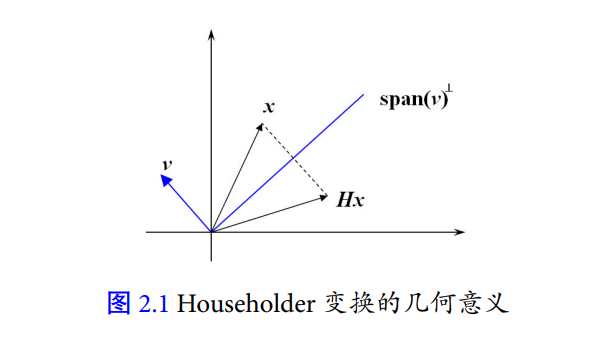
\includegraphics[scale=0.5]{figuresl/figure1.png}
\end{figure}
\end{frame}

\begin{frame}
\frametitle{Householder矩阵的几个基本性质}
\noindent \textcolor{blue}{定理}~设$H \in \mathbb{C}^{n \times n}$是一个 Householder 矩阵, 则\\
(1)$H^*=H$,即$H$ Hermite的;

(2)$H^*H=I$,即$H$是酉矩阵;

(3)$H^2=I$,所以$H^{-1}=H$;

(4)$det(H)=-1$;

(5)$H$有两个互异的特征值:$\lambda=1$和$\lambda=-1$,其中$\lambda=1$的代数重数为
$n-1$\\


\noindent Householder 矩阵的重要应用:\\
\textcolor{blue}{将一个向量除第一个元素以外的所有元素都化为零}\\



\noindent \textcolor{blue}{引理}~~设$x,y \in \mathbb{C}^n$n 为任意两个互异的向量,则存在一个Householder矩阵$H(x)$使得$y=H(v)x$的充要条件是$\|x\|_{2}=\|y\|_{2}\text{且} x^{*} y \in \mathbb{R}$(取$v=x-y$即可)
\end{frame}

\begin{frame}
\noindent\textcolor{blue}{定理}~设$x=\left[x_{1}, x_{2}, \ldots,
x_{n}\right]^{\top} \in \mathbb{R}^{n}$是一个非零向量, 则存在 Householder 矩阵
$H$使得$Hx=\alpha e_1$,其中$\alpha=\|x\|_2$(或$\alpha=-\|x\|_2$),$e_1=[1,0, \ldots, 0]^{\top} \in \mathbb{R}^{n}$

设$x=\left[x_{1}, x_{2}, \ldots, x_{n}\right]^{\top} \in \mathbb{R}^{n}$是一个实的非零向量, 下面讨论如何计算定理中的 Householder 矩阵$H(v)$. 由引理的证明过程可知$$
v=x-\alpha e_{1}=\left[x_{1}-\alpha, x_{2}, \ldots, x_{n}\right]^{\top}
$$

在实际计算中, 为了尽可能地减少舍入误差, 我们通常避免两个相近的数
做减法运算, 否则就会损失有效数字. 因此, 我通常取$$
\alpha=-\operatorname{sign}\left(x_{1}\right) \cdot\|x\|_{2}
$$

事实上,我们也可以取$\alpha=\operatorname{sign}\left(x_{1}\right)\|x\|_{2}$但此时为了减少舍入误差,我们需要通过下面的公式来计算$v$的第一个分量$v_1$
$$
\alpha=\operatorname{sign}\left(x_{1}\right)\|x\|_{2}
$$
\end{frame}

\begin{frame}
$$
v_{1}=x_{1}-\alpha=\frac{x_{1}^{2}-\|x\|_{2}^{2}}{x_{1}+\alpha}=\frac{-\left(x_{2}^{2}+x_{3}^{2}+\cdots+x_{n}^{2}\right)}{x_{1}+\alpha}
$$
$$
v_{1}=\left\{\begin{array}{ll}{x_{1}-\alpha,} & {\text { if } \operatorname{sign}\left(x_{1}\right)<0} \\ {\frac{-\left(x_{2}^{2}+x_{3}^{2}+\cdots+x_{n}^{2}\right)}{x_{1}+\alpha},} & {\text { otherwise }}\end{array}\right.
$$\\无论怎样选取$\alpha$,我们都有$H=I-\beta v v^*$其中$$
\beta=\frac{2}{v^{*} v}=\frac{2}{\left(x_{1}-\alpha\right)^{2}+x_{2}^{2}+\cdots+x_{n}^{2}}=\frac{2}{2 \alpha^{2}-2 \alpha x_{1}}=-\frac{1}{\alpha v_{1}}
$$\\
\end{frame}

\newpage
\textcolor{blue}{算法2.1}计算Householder向量\\
\textcolor{red}{\%Given~$x \in \mathbb{R}^n$,compute~$\beta$,$v$ suth that~$Hx=\|x\|_{2} e_{1}$ with $H=I-\beta v v^*$}

\begin{enumerate}[1:]
	\item function[$\beta,v$]=house($x$)
	\item $n=$ length($x$)~(here length($x$) denotes the dimension of $x$)
	\item $\sigma=x_{2}^{2}+x_{3}^{2}+\cdots+x_{n}^{2}$
	\item $v=x$
	\item if $\sigma=0$ then
	\item        \qquad if $x_1<0$ then
	\item \qquad \qquad$v_1=2x,\beta=2/v_1^2$
	\item \qquad else
	\item \qquad \qquad $v_1=0,\beta=0$
	\item\qquad end if
	\item else
	\item \qquad $\alpha=\sqrt{x_1^2+\sigma}$ ~\% $\alpha =\|x\|_2$
	\item \qquad if $x_1<0$ then
	\item \qquad \qquad $v_1=x_1-\alpha$
	\item \qquad else
	\item \qquad \qquad $v_1=-\alpha/(x_1+\alpha)$
	\item \qquad end if 
	\item \qquad $\beta=2/(v_1^2+\alpha)$
	\item end if 
\end{enumerate}

总运算量大约为 3n, 且具有很好的数值稳定性

在实际计算时, 我们可以将向量$v$单位化,使得$v_1=1$,这样,我们就无需为$v$另外分配空间,而是将$v(2:n)$存放在$x(2:n)$中, 因为变换后的向量$x$除第一个分量外, 其它都为零.

为了避免可能产生的溢出, 可事先将$x$单位化,即令$x=x/\|x\|_2$


\begin{frame}
\frametitle{Householder 变换的运算量}
设$A \in \mathbb{R}^{m \times n}, H=I-\beta v v^{*} \in \mathbb{R}^{m}$,则$$
H A=\left(I-\beta v v^{*}\right) A=A-\beta v v^{*} A=A-\beta v\left(A^{*} v\right)^{*}
$$

因此, 在做 Householder 变换时, 并不需要生成 Householder 矩阵, 只需要
Householder 向量即可. 上面矩阵相乘的总运算量大约为 4mn.
\end{frame}

\begin{frame}
\frametitle{2.4 Givens 变换}
$$G(i,j,\theta)=
\begin{bmatrix}
1& & & & & & \\
&\ddots& & & & & \\
& &c& &s& & \\
& & & \ddots& & & \\
& &-s& &c & & \\
& & & & &\ddots& \\
&&&&&&1\\
\end{bmatrix}\in \mathbb{R}^{n\times n} ~(\theta \in [0,2 \pi],i\leqslant j)
$$
Givens 变换 (或 Givens 旋转, 或 Givens 矩阵),其中$c=\cos(\theta),s=\sin (\theta)$

定理:~$G(i,j,\theta)$是正交矩阵,且det$(G(i,j,\theta))=1$\\

\noindent 左乘 Givens 矩阵: 只会影响第$i$行和第$j$的元素.\\
右乘 Givens 矩阵: 只会影响第 i 和第 j 列的元素.
\end{frame}

\begin{frame}
例 ~ 设$x=\left[x_{1}, x_{2}\right]^{\top} \in \mathbb{R}^{2}$,, 则存在一个 Givens 变换$G=\left[\begin{array}{cc}{c} & {s} \\ {-s} & {c}\end{array}\right] \in \mathbb{R}^{2 \times 2}$使得$G x=[r, 0]^{\top}$,其中$c,s$和$r$的值如下:

\begin{itemize}
	\item {若$x_1=x_2=0$,则$c=1,s=0,r=0$;}
	\item{若$x_1=0$但$x_2\ne0$,则$c=0,s=x_2/\left|x_2\right|,r=\left|x_2\right|$}
	\item 若$x_1\ne 0$但$x_2=0$,则$c=$sign$(x_1),s=0,r=\left|x_1\right|$;
	\item 若$x_1\ne 0$且$x_2\ne 0$,则$c=x_1/r,s=x_2/r,r=\sqrt{x_1^2+x_2^2}$.
\end{itemize}
通过 Givens 变换, 我们可以将向量$x \in \mathbb{R}^2$的第二个分量化为 0.

事实上, 对于任意一个向量$x \in \mathbb{R}^n$,我们都可以通过 Givens 变换将其任意一个位置上的分量化为 0. 更进一步, 我们也可以通过若干个 Givens 变换, 将$x$中除第一个分量外的所有元素都化为 0.
\end{frame}

\begin{frame}
\noindent \textcolor{blue}{算法2.2}Givens变换\\
\textcolor{red}{\%~Given~$x=[a,b]^{\top}$,compute~$c$,$s$~such that~$Gx=[r,0]^{\top}$~where~$r=\|x\|_2$}
\begin{enumerate}[1:]
	\item function~$[c,s]$ = givens$(a,b)$
	\item if $b=0$ then
	\item \qquad if $a \ge 0$then
	\item \qquad \qquad $c=1,s=0$
	\item \qquad else
	\item \qquad \qquad $c=-1,s=0$
	\item \qquad end if
	\item else
	\item \qquad if $|b|>|a|$ then
	\item \qquad \qquad $\tau=a / b, \quad s=\operatorname{sign}(b) / \sqrt{1+\tau^{2}}, \quad c=s \tau$
	\item \qquad else
	\item \qquad \qquad $\tau=b / a, \quad c=\operatorname{sign}(a) / \sqrt{1+\tau^{2}}, \quad s=c \tau$
	\item \qquad end if
	\item end if  
\end{enumerate}
\end{frame}

\begin{frame}
\frametitle{2.5 正交变换的舍入误差分析}
\noindent \textcolor{blue}{引理}~设$P \in \mathbb{R}^{n \times n}$是一个精确的 Householder 或 Givens 变换, $\tilde P$是其浮点运算近似, 则$$
\mathrm{fl}(\tilde{P} A)=P(A+E), \quad \mathrm{fl}(A \tilde{P})=(A+F) P
$$\\
其中$\|E\|_{2}=\mathcal{O}\left(\varepsilon_{u}\right) \cdot\|A\|_{2},\|F\|_{2}=\mathcal{O}\left(\varepsilon_{u}\right) \cdot\|A\|_{2}$\\

\noindent 这说明对一个矩阵做 Householder 变换或 Givens 变换是向后稳定的.

考虑对矩阵$A$做一系列的正交变换, 则有$$
\mathrm{fl}\left(\tilde{P}_{k} \cdots \tilde{P}_{1} A \tilde{Q}_{1} \cdots \tilde{Q}_{k}\right)=P_{k} \cdots P_{1}(A+E) Q_{1} \cdots Q_{k}
$$\\其中$\|E\|_{2}=\mathcal{O}\left(\varepsilon_{u}\right) \cdot\left(k\|A\|_{2}\right)$,这说明整个计算过程是向后稳定的
\end{frame}

\begin{frame}
一般地, 假设$X$是一个非奇异的线性变换, $\tilde{X}$是其浮点运算近似. 当$X$作用到$A$上时, 我们有$$
\mathrm{fl}(\tilde{X} A)=X A+E=X\left(A+X^{-1} E\right) \triangleq X(A+F)
$$\\
其中$\|E\|_{2}=O\left(\varepsilon_{u}\right) \cdot\|X A\|_{2} \leq O\left(\varepsilon_{u}\right) \cdot\|X\|_{2} \cdot\|A\|_{2}$,故$$
\|F\|_{2}=\left\|X^{-1} E\right\|_{2} \leq \mathcal{O}\left(\varepsilon_{u}\right) \cdot\left\|X^{-1}\right\|_{2} \cdot\|X\|_{2} \cdot\|A\|_{2}=\mathcal{O}\left(\varepsilon_{u}\right) \cdot \kappa_{2}(X) \cdot\|A\|_{2}
$$\\
因此, 舍入误差将被放大$k_2(X)$倍. 当$X$是正交变换时,$k_2(X)$达到最小
值 1, 这就是为什么在浮点运算中尽量使用正交变换的原因.
\end{frame}
\section{QR分解}
\begin{frame}
\frametitle{3 QR分解}
\begin{enumerate}[3.1]
	\item \textcolor{blue}{QR分解的存在唯一性}
	\item \textcolor{blue}{基于MGS的QR分解}
	\item \textcolor{blue}{基于 Householder 变换的 QR 分解}
	\item \textcolor{blue}{列主元 QR 分解}
	\item \textcolor{blue}{基于 Givens 变换的 QR 分解}
	\item \textcolor{blue}{QR 分解的稳定性}
\end{enumerate}
\end{frame}

\begin{frame}
\frametitle{3.1 QR分解的存在唯一性}
\textcolor{blue}{定理(QR分解)}~设$A \in \mathbb{C}^{m \times n}(m \geq n)$.则存在一个单位列正交矩阵$Q \in \mathbb{C}^{m \times n}$和一个上三角矩阵$R \in \mathbb{C}^{n \times n}$,使得
\begin{eqnarray}
A=QR
\end{eqnarray}
\textcolor{blue}{证明}:设$A=\left[a_{1}, a_{2}, \ldots, a_{n}\right] \in \mathbb{C}^{m \times n}$\\
若$A$列满秩, 即 rank($A$) = $n$. 则 QR 分解(4)就是对$A$的列向量组进行
Gram-Schmidt 正交化过程的矩阵描述. 具体过程见下面的算法.
\end{frame}

\begin{frame}
\textcolor{blue}{算法3.1} Gram-schmidt Process\\
\begin{enumerate}[1:]
	\item $r_{11}=||a_{1}||_{2}$
	\item $q_{1}=a_{1}/r_{11}$
	\item  for $j = 2$ to n do
	\item  \qquad $q_{j}=a_{j}$
	\item  \qquad for $i=1$ to $j-1$ do
	\item  \qquad \qquad $r_{ij}=q_{i}^{*}a_{j}$
	\item  \qquad \qquad $q_{j}=q_{j}-r_{ij}q_{i}$
	\item \qquad end for
	\item \qquad $r_{jj}=||q_{j}||_{2}$
	\item \qquad $q_{j}=q_{j}/r_{jj}$
	\item end for
\end{enumerate}
\end{frame} 

\begin{frame}
如果A不是列满秩,我们可以做类似的正交化过程:
\begin{itemize}
	\item 如果$a_1=0$则令$q_1=0$;否则令$q_1=a_1/||a_1||_2$;
	\item 对于$j=2,3,\cdots$计算$\tilde{q}_{j}=a_j-\sum_{i=1}^{j-1}(q_i^*a_j)q_i$.\\
	如果$\tilde{q_j}=0$则令$q_j=0$,否则令$q_j=\tilde{q_j}/||\tilde{q_j}||_2$\\
\end{itemize}
于是我们有
\[
A=QR
\]
其中$Q=[q_1,q_2,...,q_n]$列正交(但不是单位列正交,列向量中可能有零向量).这里的$R=[r_{ij}]_{n\times n}$是上三角矩阵,定义如下
\[
r_{ij}=
\begin{cases}
q_{i}^{*} a_{j},&for i\leq j\\
0,&for i>j
\end{cases}
\]
\textcolor{blue}{易知,如果Q的某一列$q_k=0$,则R中对应的第k行全为0}
\end{frame}

\begin{frame}
设$rank(A)=l<n$,则rank$(Q)=l$即Q只有$l$个非零列,不妨设为$ q_{i1},q_{i2},...q_{il} $,他们构成$ \mathbb{C}^m $的一个单位正交向量组,将其扩展成$ \mathbb{C}^m $中的一组标准正交基,即
\[
q_{i_1},q_{i_2},...q_{i_l},\tilde{q}_1,,...\tilde{q}_{m-l}
\]
然后我们用$ \tilde{q_1} $ 替换Q中的第一个零列,用$ \tilde{q}_2 $	替换Q总的第二个零列,依次类推,将Q中的所有零列都替换掉.将最后得到的矩阵记为$\tilde{Q}$,于是$\tilde{Q}\in\mathbb{C}^{m\times n}$ 单位列正交. \textcolor{blue}{由于$\tilde{Q}$中的新添加的列向量正好与$R$中的零行相对应},所以
\[
\tilde{Q}R=QR=A
\]
这就是~$A$~的~$QR$~分解
\end{frame}


\begin{frame}
\frametitle{满秩矩阵QR分解的存在唯一性}
\textcolor{blue}{定理} 若A列满秩,并要求R的对角线元素都为正,则A的QR分解存在且唯一.\\

$\dagger$若A是实矩阵,则所有运算都是实运算,因此Q和R都是实矩阵.\\

$\dagger$有时也将QR分解定义为:存在酉矩阵$Q\in\mathbb{C}^{m\times m}$使得
\[
A = A\begin{bmatrix}R_{11}\\0\end{bmatrix}
\]
其中$R_{11}\in\mathbb{R}^{n\times n}$为上三角矩阵.
\end{frame}

\begin{frame}
若$A$不满秩,存在置换矩阵$P$,使得$AP$的前$l$列
线性无关,其中$l=rank(A)$.对$AP$进行$QR$分解,可得:\\
\textcolor{blue}{推论} ~设$A\in\mathbb{C}^{m\times n}(m\geq n)$ 则存在一个置换矩阵$P$,使得
\[
AP=Q\begin{bmatrix}R_{11}&R_{12}\\0&0\end{bmatrix}_{n\times n}
\]
其中$Q\in\mathbb{C}^{m\times n}$单位列正交,$R_{11}\in\mathbb{C}^{l\times l}$是非奇异上三角矩阵.\\
$\dagger$上述结论可简化为
\[
AP=Q\begin{bmatrix}R_{11}&R_{12}\end{bmatrix}
\]
其中$Q\in\mathbb{C}^{m\times n}$单位列正交,$R_{11}\in\mathbb{C}^{l\times l}$是非奇异上三角
\end{frame}

\begin{frame}
\textcolor{blue}{推论(满秩分解)}~设$A\in\mathbb{C}^{m\times n}$,且$rank(A)=l\le min\{m,n\}$, 则存在满秩矩阵$F\in\mathbb{C}^{m\times l}$和$G\in\mathbb{C}^{l\times n}$ ,使得
\[
A=FG
\]

$\dagger$如果A是非奇异方阵,则QR分解可用来求解线性方程组$Ax=b$\\

$\dagger$基于G-S正交化的QR分解的运算量大约为$2mn^{2}$.\\

在后面,我们会介绍基于Householder变换的QR分解,在不需要计算Q的情况下,运算量大约为$2mn^{2}-2n^{3}/3$,如果需要计算Q,则需另外大约$2mn^{2}-2n^{3}/3$运算量.
\end{frame}

\begin{frame}
\frametitle{3.2 基于MGS的QR分解}
由于数值稳定性方面的原因,在实际计算中,我们一般不采用Gram-Schmidt过程,取而代之的是修正的是\textcolor{blue}{Gram-Schmidt过程},本算法的运算量大约为$2mn^{2}$
\end{frame}

\newpage
\textcolor{blue}{算法3.2}~基于MGS的QR分解\\
\textcolor{red}{\% Given $A \in \mathbb{R}^{m\times n}$, compute $Q = [q_{1},...,q_{n}]$ and R such that $A = QR$}\\
\begin{enumerate}
	\item Set $R=[r_{ik}]=0_{n\times n}$(the $n\times n$zero matrix)
	\item if $a_{1}=0$ then 
	\item \qquad $q_{1}=0$
	\item else
	\item \qquad $r_{11}=||a_{1}||_{2}$
	\item \qquad $q_{1}=a_{1}/||a_{1}||_{2}$
	\item end if
	\item for $k=2$ to n do
	\item \qquad $q_{k} = a_{k}$
	\item \qquad for $i = 1$ to $k-1$ do
	\item \qquad \qquad $r_{ik}=q_{i}^{T}q_{k}$
	\item \qquad \qquad $q_{k}=q_{k}-r_{ik}q_{i}$
	\item \qquad end for 
	\item \qquad if $q_{k}\ne 0$ then
	\item \qquad \qquad $r_{kk}=||q_{k}||_{2}$
	\item \qquad \qquad $q_{k}=q_{k}/r_{kk}$
	\item \qquad end if
	\item end for  
\end{enumerate}
$\dagger$ MGS 得到的QR分解中,$Q\in\mathbb{R}^{n\times n},R\in\mathbb{R}^{n\times n}$

\begin{frame}
\frametitle{3.3 基于Householder变换的OR分解}
由Householder变换的性质可知,我们可以将任何一个非零变量$x\in\mathbb{R}^{n}$转化成$||x||_{2}e_{1}$,即除第一个元素外,其他都为零.\\
假定$m=n$,即$A\in\mathbb{R}^{n\times n}$ 令$H_{1}\in\mathbb{R}^{n\times n}$为Householder变换,满足
$$
H_{1}\left[\begin{array}{c}{a_{11}} \\ {a_{21}} \\ {\vdots} \\ {a_{n 1}}\end{array}\right]=\left[\begin{array}{c}{r_{1}} \\ {0} \\ {\vdots} \\ {0}\end{array}\right]
$$
于是
$$
H_{1} A=\left[\begin{array}{c|ccc}
{r_{1}}&{\tilde{a}_{12}} &\cdots& {\tilde{a}_{1 n}} \\ \hline 
0& & & \\
\vdots&&{\tilde{A}_{2}}& \\
0& & &\\
\end{array}\right],\tilde{A}_{2} \in \mathbb{R}^{(n-1) \times(n-1)}
$$
\end{frame}

\begin{frame}
同样,构造Householder变换$\tilde{H}_{2} \in \mathbb{R}^{(n-1) \times(n-1)}$,使得
$$
\tilde{H}_{2} \tilde{A}_{2}=\left[\begin{array}{c|ccc}
{r_{1}}&{\tilde{a}_{12}} &\cdots& {\tilde{a}_{1 n}} \\ \hline 
0& & & \\
\vdots&&{\tilde{A}_{2}}& \\
0& & &\\
\end{array}\right],\tilde{A}_{2} \in \mathbb{R}^{(n-1) \times(n-1)}
$$
令$H_{2}=\left[\begin{array}{cc}{1} & {0} \\ {0} & {\tilde{H}_{2}}\end{array}\right] \in \mathbb{R}^{n \times n}$,则
$$
H_{2} H_{1} A=
\left[\begin{array}{cc|ccc}
{r_{1}} & {\tilde{a}_{12}} & {\tilde{a}_{13}} & {\cdots} &{\tilde{a}_{1 n}} \\ 
{0} & {r_{2}} & {\tilde{a}_{23}}& {\cdots} & {\tilde{a}_{2 n}} \\ 
\hline 
0 & {0} &   &  &  \\
\vdots&\vdots& &{\tilde{A}_{3}}  & \\
{0} & {0} & {} & & \end{array}\right]
$$
\end{frame}

\begin{frame}
不断重复上述过程,这样,我们就得到一系列的矩阵
$$
H_{k}=\left[\begin{array}{cc}{I_{k-1}} & {0} \\ {0} & {\tilde{H}_{k}}\end{array}\right], \quad k=2,3, \ldots, n-1
$$
使得
$$
H_{n-1} \cdots H_{2} H_{1} A=\left[\begin{array}{cccc}{r_{1}} & {\tilde{a}_{12}} & {\cdots} & {\tilde{a}_{1 n}} \\ {0} & {r_{2}} & {\cdots} & {\tilde{a}_{2 n}} \\ {\vdots} & {} & {\ddots} & {\vdots} \\ {0} & {0} & {\cdots} & {r_{n}}\end{array}\right] \triangleq R
$$
令$Q=\left(H_{n-1} \cdots H_{2} H_{1}\right)^{-1}=H_{1} H_{2} \cdots H_{n-1}$,则
$$
A=\left(H_{n-1} \cdots H_{2} H_{1}\right)^{-1} R=Q R
$$
\textcolor{blue}{如果不需要生成Q,则运算量大约为$2mn^{2}-2/3n^{3}$}.\end{frame}

\begin{frame}
\frametitle{矩阵$Q$的计算}
可通过下面的算法实现
$$
Q=I_{n}, \quad Q=Q H_{k}, \quad k=1,2, \ldots, n-1
$$
若保留了所有的Householder向量,则Q可以通过下面的\textcolor{blue}{向后累积法}实现:
$$
Q=I_{n}, \quad Q=H_{k} Q, \quad k=n-1, n-2, \ldots, 1
$$
\textcolor{blue}{优点:一开始Q会比较稀疏,随着迭代的进行,Q才会慢慢变满}\\
运算量大约为$4(m^{2}n-mn^{2}+\frac{1}{3}n^{3})$.\\
$\dagger$若$m>n$ 则由Householder变换得到的QR分解中,$Q\in\mathbb{R}^{m\times m},R\in\mathbb{R}^{m\times n}$
\end{frame}

\begin{frame}
\noindent \textcolor{blue}{算法3.3}基于Householder变换的QR分解\\
\textcolor{red}{\%Given$A \in \mathbb{R}^{m×\times n}$,compute$Q \in \mathbb{R}^{m\times m}$,$R\in \mathbb{R}^{m\times n}$ such that $A = QR$ \% The upper triangular part of R is stored in the upper triangular part of A}
\begin{enumerate}[1:]
	\item Set $Q=I_{m\times m}$
	\item for $k=1$ to n do
	\item \qquad $x=A(k:m,k)$
	\item \qquad$[\beta, v_{k}]$ = house(x)
	\item \qquad$v_{k} = v_{k}||v||2$
	\item \qquad$A(k:m,k:n)=(I_{m-k+1} −2v_{k}v_{k}^{T})A(k:m,k:n)$
	\item \qquad$Q(1:k−1,k:m)=Q(1:k−1,k:m)(I_{m−k+1} -2v_{k}v_{k}^{⊺})$
	\item \qquad$Q(k:m,k:m)=Q(k:m,k:m)(I_{m−k+1} -2v_{k}v_{k}^{T})$
	\item end for
\end{enumerate}
\textcolor{blue}{上面的算法只是一个简单描述, 并没有考虑运算量问题}.
\end{frame}

\begin{frame}
$\dagger$在实际计算时, 我们通常会保留所有的 Householder 向量.\\

由于第k步中$\hat{H}_{k}$ 所对应的Householder向量$v_{k}$ 的长度为$m−k+1$, 因此我们先把 $v_{k}$ 单位化, 使得 $v_{k}$ 的第一元素为 1, 这样就只要存储 $v_{k}(2:end)$, 共 $m - k$ 个元素.\\

\textcolor{blue}{这样, 我们就可以把所有的 Householder 向量存放在 A 的严格下三 角部分, 而 A 的上三角部分仍然存放 R.}\\

在计算 Q 时采用向后累积的方法, 所以总的运算量大约为 $4m^{2}n - 2mn^{2} + 2n^{3}$. 若 $m = n$, 则运算量大约为 $8n^{3}$.\\

$\dagger$我们也可以考虑分块 Householder QR 分解, 以便充分利用 3 级 BLAS 运算, 提高计算效率.
\end{frame}


\begin{frame}
\frametitle{3.4 列主元QR分解}
\noindent 当 A 不是满秩时, 我们可以进行\textcolor{blue}{列主元 QR 分解.}\\
\textcolor{blue}{定理(列主元QR分解)}~设$A \in \mathbb{C}^{m \times n}(m \geq n)$,且$\operatorname{rank}(A)=k<n$,则存在置换矩阵 P, 正交矩阵$Q \in \mathbb{C}^{m \times m}$,使得
$$
A P=Q\left[\begin{array}{cc}{R_{11}} & {R_{12}} \\ {0} & {0}\end{array}\right]_{m \times n}
$$
其中$R_{11} \in \mathbb{C}^{k \times k}$是非奇异上三角矩阵,且对角线元素满足$r_{11} \geq r_{22} \geq \cdots \geq r_{k k}>0$\\

列主元 QR 分解的实现过程与 QR 分解基本类似, 只是每一步需要选个列 主元, 同时做一个列交换
\end{frame}

\begin{frame}
假设经过$l$步后,我们得到下面的分解
$$
A P^{(l)}=Q^{(l)}\left[\begin{array}{cc}{R_{11}^{(l)}} & {R_{12}^{(l)}} \\ {0} & {R_{22}^{(l)}}\end{array}\right] \triangleq Q^{(l)} R^{(l)},\text 或\left(Q^{(l)}\right)^{\top} A P^{(l)}=R^{(l)}
$$
其中$P^(l)$为置换矩阵,$Q^(l)$为正交矩阵,$R_{12}^{(l)} \in \mathbb{R}^{(l) \times(l)}$非奇异上三角矩阵.\\
下面进行第$l+1$步:
\begin{enumerate}
	\item 计算 $R_{22}^{(l)}$ 所有列的范数, 若都为 0, 则算法结束, 此时必有 $l = k$.
	\item 若$l < k$,则$R_{22}^{(l)}\ne 0$. 设范数最大的列为第$i_{l+1}$列(若有相等的,取其中一列即可), 范数为 $r_{l+1,l+1}$. 若 $i_{l+1}\ne 1$, 则交换 $R(l)$ 的第 $l + 1$ 列与第 $i_{l+1} + l$ 列, 并记相应的置换矩阵为 $P_{l+1}$.
	\item 以 $R_{22}^{(l)}$ 的第 1 列构造 Householder 变换 $\bar{H}_{l+1}$\\
	令$H_{l+1}=Blkdiag(I_{l},\bar{H}_{l+1}),P^{(l+1)}=P^{(l)} P_{l+1}$.则
\end{enumerate}
$$
H_{l+1}\left(Q^{(l)}\right)^{\top} A P^{(l+1)}=H_{l+1} R^{(l)} P_{l+1}=\left[\begin{array}{cc}{R_{11}^{(l)}} & {\tilde{R}_{12}^{(l)}} \\ {0} & {\tilde{R}_{22}^{(l)}}\end{array}\right] \triangleq R^{(l+1)}
$$
\end{frame}

\begin{frame}
其中 $\tilde {R}_{22}^{(l)}$ 的第一列除第一个元素外, 其余都是零, 且该元素等于$r_{l+1,l+1}$,即
$$
R^{(l+1)}=\left[\begin{array}{c c |c c}{R_{11}^{(l)}} & {*} & {*} \\ {0} & {r_{l+1, l+1}} & {*} \\ \hline {0} & {0} & {*}\end{array}\right] \triangleq\left[\begin{array}{cc}{R_{11}^{(l+1)}} & {R_{12}^{(l+1)}} \\ {0} & {R_{22}^{(l+1)}}\end{array}\right]
$$
其中$R_{11}^{(l+1)} \in \mathbb{R}^{(l+1) \times(l+1)}$为非奇异上三角矩阵\\
记$Q^{(l+1)} \triangleq Q^{(l)} H_{l+1}^{\top}$,则
$$
A P^{(l+1)}=Q^{(l+1)} R^{(l+1)}
$$
依此类推, 直到第 k 步, 即可得 A 的列主元 QR 分解.\\
矩阵 R11 的对角线元素的递减关系可由列主元的选取方法推出.
\end{frame}

\begin{frame}
\frametitle{3.5 基于Givens变换的QR分解}
我们同样可以利用 Givens 变换来做 QR 分解.\\
设$A \in \mathbb{R}^{n \times n}$,构造 Givens 变换 $G_{21}$, 作用在 A 的最前面的两行上, 使得
$$
G_{21}\left[\begin{array}{c}{a_{11}} \\ {a_{21}} \\ {a_{31}} \\ {\vdots} \\ {a_{n 1}}\end{array}\right]=\left[\begin{array}{c}{\tilde{a}_{11}} \\ {0} \\ {a_{31}} \\ {\vdots} \\ {a_{n 1}}\end{array}\right]
$$
构造Givens变换$G_{31}$,作用在$G_{21}A$的第1行和第3行上,将$a_{31}$ 化为零. 由于 $G_{31}$ 只改变第 1 行和第 3 行的值, 所以第二行的零元素维持不变.
\end{frame}

\begin{frame}
以此类推, 我们可以构造一系列的 Givens 变换 $G_{41}, G_{51}, \ldots, G_{n 1}$ 使得 $G_{n 1} \cdots G_{21} A$ 的第一列中除第一个元素外, 其它元素都化为零, 即
$$
G_{n 1} \cdots G_{21} A=
\left[\begin{array}{cccc}
{*} & {*} & {\cdots} & {*} \\ 
{0} & {*} & {\cdots} & {*} \\ 
{\vdots} & {\vdots} & & {\vdots} \\ 
{0} & {*} & {\cdots} & {*}
\end{array}\right]
$$
下面我们可以对第二列进行类似的处理.构造Givens变换$G_{32},G_{42},\ldots, G_{n 2}$将第二列的第 3 至第 n 个元素全化为零, 同时保持第一列不变. \\
其他列也做类似的处理. 最后, 通过构造$\frac{1}{2} n(n-1)$个 Givens 变换, 将转化成一个上三角矩阵$R$, 即
$$
R=G_{n, n-1} \cdots G_{21} A,\text 或A=\left(G_{n, n-1} \cdots G_{21}\right)^{\top} R \triangleq Q R
$$
\end{frame}

\begin{frame}
$\dagger$与 Householder 变换一样, 在进行 Givens 变换时, 我们不需要显式地 写出 Givens 矩阵.\\
$\dagger$对于稠密矩阵而言, 基于 Givens 变换的 QR 分解的运算量比 House- holder 变换要多很多.\\
\textcolor{blue}{基于 Givens 变换的 QR 分解主要用于当矩阵的非零下三角元素相对 较少时的情形, 比如对上 Hessenberg 矩阵进行 QR 分解}\\
$\dagger$如果 $A \in \mathbb{R}^{m\times n}, m > n$, 仍然可以通过 Givens 变换进行 QR 分解
\end{frame}

\begin{frame}
\textcolor{blue}{算法3.4:}基于 Givens 变换的 QR 分解\\
\textcolor{red}{\%Given $A \in \mathbb{R}^{m\times n}$,compute$Q \in \mathbb{R}^{m×\times m}$ and$R\in \mathbb{R}{m\times n}$ such that $A = QR$\\
	\% The upper triangular part of R is stored in the upper triangular part of A}
\begin{enumerate}[1:]
	\item Set $Q=I_{m\times m}$
	\item for $k=1$ to n do
	\item \qquad for i = k + 1 to m do
	\item \qquad \qquad $[c, s]=givens(a_{kk}, a_{ik})$
	\item \qquad \qquad $\left[\begin{array}{c}{A(k, k : n)} \\ {A(i, k : n)}\end{array}\right]=G\left[\begin{array}{c}{A(k, k : n)} \\ {A(i, k : n)}\end{array}\right]$ where $G=\left[\begin{array}{cc}{c} & {s} \\ {-s} & {c}\end{array}\right]$
	\item \qquad \qquad $[Q(1 : m, k), Q(1 : m, i)]=[Q(1 : m, k), Q(1 : m, i)] G^{\top}$
	\item \qquad end for
	\item end for
\end{enumerate}
\end{frame}

\begin{frame}
\frametitle{3.6 QR分解的稳定性}
\noindent 基于 Householder 变换和 Givens 变换的 QR 分解都具有很好的数值稳定性, 基于 MGS 的 QR 分解也是向后稳定的\\
$\dagger$如果需要计算 Q, 则 MGS 的运算量相对较少, 因此当 A 的列向量具有很好的线性无关性时, 我们可以使用 MGS 来计算 QR 分解.\\
Björck [Björck 1967] 证明了, 通过 MGS 计算的矩阵 Q 满足
$$
Q^{\top} Q=I+E_{M G S},~~\left\|E_{M G S}\right\|_{2} \approx \varepsilon_{u} \kappa_{2}(A)
$$
而 Householder 变换计算的矩阵 Q 满足
$$
Q^{\top} Q=I+E_{H},~~\left\|E_{H}\right\|_{2} \approx \varepsilon_{u}
$$
因此, 如果正交性至关重要, 建议使用 Householder 变换, 特别是当 A 的列 向量接近线性相关时
\end{frame}
\section{奇异值分解}
\begin{frame}
\frametitle{4 奇异值分解}
\textcolor{blue}{定理(SVD)}设$A \in \mathbb{C}^{m \times n}(m \geq n)$则存在酉矩阵$U \in \mathbb{C}^{m \times m}$和$V \in \mathbb{C}^{n \times n}$,使得
\begin{equation}
U^{*} A V=\left[\begin{array}{l}{\Sigma} \\ {0}\end{array}\right],orA=U\left[\begin{array}{l}{\Sigma} \\ {0}\end{array}\right] V^{*}
\end {equation}
其中$\Sigma=\operatorname{diag}\left(\sigma_{1}, \sigma_{2}, \ldots, \sigma_{n}\right) \in \mathbb{R}^{n \times n}$,且$\sigma_{1} \geq \ldots \geq \sigma_{n} \geq 0$\\

$\dagger$该定理也可以通过 Hermite 半正定矩阵的特征值分解来证明.\\

\textcolor{blue}{定义} 分解(3.6)称为$A$的\textcolor{blue}{奇异值分解(SVD)},$\sigma_{1}, \sigma_{2}, \dots, \sigma_{n}$称为A的奇 异值, 它们是矩阵 $A^{*}A$ 的特征值的平方根.
\end{frame}

\begin{frame}
$\dagger$在不做特别说明的情况下,我们总是假定$\sigma_{1} \geq \sigma_{2} \geq \cdots \geq \sigma_{n} \geq 0$\\
$\dagger$如果$A \in \mathbb{R}^{m \times n}$是实矩阵, 则U,V也都可以是实矩阵

\noindent 奇异向量\\
矩阵$U=\left[u_{1}, u_{2}, \ldots, u_{m}\right]$和$V=\left[v_{1}, v_{2}, \ldots, v_{n}\right]$的列向量分别称为 A 的\textcolor{blue}{左奇异向量}和\textcolor{blue}{右奇异向量}, 即存在关系式
$$
\begin{array}{l}{A v_{i}=\sigma_{i} u_{i}, \quad i=1,2, \ldots, n} \\ {A^{*} u_{i}=\sigma_{i} v_{i}, \quad i=1,2, \ldots, n} \\ {A^{*} u_{i}=0, \quad i=n+1, n+2, \ldots, m}\end{array}
$$
\end{frame}

\begin{frame}
\frametitle{SVD的其他形式}
$$
A=U\left[\begin{array}{l}{\Sigma} \\ {0}\end{array}\right] V^{*}=\sigma_{1} u_{1} v_{1}^{*}+\sigma_{2} u_{2} v_{2}^{*}+\cdots+\sigma_{n} u_{n} v_{n}^{*}
$$
记$U_{n}=\left[u_{1}, u_{2}, \ldots, u_{n}\right] \in \mathbb{C}^{m \times n}$,则$U_{n}$是单位列正交矩阵,且
\begin{equation}
A=U_{n} \Sigma V^{*}
\end{equation}
这就是所谓的细 SVD (thin SVD ) 或 降阶 SVD (reduced SVD ), 有的文献 将上式称为奇异值分解.\\
当$k < n$时,我们称
$$
A_{k}=\sigma_{1} u_{1} v_{1}^{*}+\sigma_{2} u_{2} v_{2}^{*}+\cdots+\sigma_{k} u_{k} v_{k}^{*}
$$
为 A 的截断 SVD (truncated SVD ).
\end{frame}

\begin{frame}
\frametitle{奇异值基本性质}
\textcolor{blue}{定理:}设$A=U\left[\begin{array}{l}{\Sigma} \\ {0}\end{array}\right] V^{*}$是$A \in \mathbb{C}^{m \times n}(m \geq n)$的奇异值分解,则
\begin{enumerate}[(1)]
	\item $A^{*} A$ 的特征值是 $\sigma_{i}^{2}$ , 对应的特征向量是 $v_{i}$
	\item $AA^{*}$的特征值是$\sigma_{i}^{2}$和$m-n$个零,对应的特征向量是$u_{i}$
	\item $\|A\|_{2}=\sigma_{1},\|A\|_{F}=\sqrt{\sigma_{1}^{2}+\sigma_{2}^{2}+\cdots+\sigma_{n}^{2}}$
	\item 若$\operatorname{rank}(A)=r \leq n$,则$\operatorname{Ran}(A)=\operatorname{span}\left\{u_{1}, u_{2}, \ldots, u_{r}\right\}$,$\operatorname{Ker}(A)=\operatorname{span}\left\{v_{r+1}, v_{r+2}, \ldots, v_{n}\right\}$
	\item 设$x \in \mathbb{C}^{n}$,且$\|x\|_{2}=1$和$Y \in \mathbb{C}^{n \times n}$是酉矩阵,则$\sigma_{i}\left(X^{*} A Y\right)=\sigma_{i}(A)$
	\item (酉不变性)$X \in \mathbb{C}^{m \times m}$和$Y \in \mathbb{C}^{n \times n}$是酉矩阵,则$\sigma_{i}\left(X^{*} A Y\right)=\sigma_{i}(A)$
\end{enumerate}
\end{frame}

\begin{frame}
\textcolor{blue}{定理} 设$A=U \Sigma V^{*}$是$A \in \mathbb{C}^{n \times n}$的奇异值分解,则:
\begin{enumerate}[(1)]
	\item $|\operatorname{det}(A)|=\sigma_{1} \sigma_{2} \cdots \sigma_{n}$
	\item 若A非奇异,则$\left\|A^{-1}\right\|_{2}=\sigma_{n}^{-1}, \kappa_{2}(A)=\sigma_{1} / \sigma_{n}$
	\item 若A是Hermite的,且$A=U \Lambda U^{*}$是A的酉特征值分解,设$\left|\lambda_{1}\right| \geq\left|\lambda_{2}\right| \geq \cdots \geq\left|\lambda_{n}\right|$,则$A=U \Sigma V$是A的奇异值分解,其中$\sigma_{i}=\left|\lambda_{i}\right|, v_{i}=\operatorname{sign}\left(\lambda_{i}\right) u_{i}$,若$\lambda_{i}=0$,则$v_{i}=u_{i}$
	\item 矩阵$\left[\begin{array}{cc}{0} & {A^{*}} \\ {A} & {0}\end{array}\right]$的特征值是$\pm \sigma_{i}$,对应单位特征向量$\frac{1}{\sqrt{2}}\left[\begin{array}{c}{v_{i}} \\ { \pm u_{i}}\end{array}\right]$
\end{enumerate}
$\dagger$矩阵条件数取决于奇异值, 不是特征值, 见讲义上的例子
\end{frame}

\begin{frame}
\frametitle{低秩逼近}

\textcolor{blue}{定理}设$A=U_{n} \Sigma V^{*}$是$A \in \mathbb{C}^{m \times n}$的奇异值分解. 令
$$
A_{k}=\sum_{i=1}^{k} \sigma_{i} u_{i} v_{i}^{*}
$$
则$A_{k}$是
\begin{equation}
\min _{B \in \mathbb{C}^{m \times n}, \operatorname{rank}(B)=k}\|A-B\|_{2}
\end{equation}
的一个解, 且
$$
\left\|A-A_{k}\right\|_{2}=\sigma_{k+1}
$$
此时,我们称Ak 是A的一个\textcolor{blue}{秩k逼近}\\
$\dagger$对于 Frobenius 范数, 我们有类似的结论.(\textcolor{blue}{证明留作练习})
\end{frame}

\begin{frame}
\textcolor{blue}{定理(Weyl)}设$A, B \in \mathbb{C}^{m \times n}(m \geq n)$且$\operatorname{rank}(B)=k$,则有
\begin{equation}
\max _{x \in \operatorname{Ker}(B),\|x\|_{2}=1}\|A x\|_{2} \geq \sigma_{k+1}(A)
\end{equation}
和
\begin{equation}
\min _{x \in \operatorname{Ker}(B),\|x\|_{2}=1}\|A x\|_{2} \leq \sigma_{n-k}(A)
\end{equation}
因此,
\begin{equation}
\sigma_{1}(A-B) \geq \sigma_{k+1}(A), \quad \sigma_{n}(A+B) \leq \sigma_{n-k}(A)
\end{equation}
且
\begin{equation}
\sigma_{i+j-1}(A) \leq \sigma_{i}(B)+\sigma_{j}(A-B), \quad i=1,2, \ldots, n, j=1,2, \ldots, n-i+1
\end{equation}
\end{frame}

\begin{frame}
根据 Weyl 定理, 我们可以得到矩阵奇异值的最小最大定理.\\

\textcolor{blue}{定理}设$\sigma_{1} \geq \sigma_{2} \geq \cdots \geq \sigma_{n} \geq 0$是矩阵$A \in \mathbb{C}^{m \times n}(m \geq n)$的奇异值,则
$$
\sigma_{k}(A)=\min _{\operatorname{dim}(\mathcal{L})=n-k+1} \max _{x \in \mathcal{L},\|x\|_{2}=1}\|A x\|_{2}, \quad k=1,2, \ldots, n
$$
和
$$
\sigma_{k}(A)=\max _{\operatorname{dim}(\mathcal{L})=k} \min _{x \in \mathcal{L},\|x\|_{2}=1}\|A x\|_{2}, \quad k=1,2, \ldots, n
$$
其中$\mathcal{L}$表示$\mathbb{C}^{n}$ 的一个子空间.
\end{frame}

\begin{frame}
\textcolor{blue}{引理(交错不等式)}设$A \in \mathbb{C}^{m \times n}, A_{r}$是由A去除r列(或r行)后得到的子矩阵,则
$$
\sigma_{i}(A) \geq \sigma_{i}\left(A_{r}\right) \geq \sigma_{i+r}(A), \quad i=1,2, \ldots, \min \{m, n\}
$$
这里, 当下标 k 大于矩阵的维数时, 我们令 $\sigma_{k} = 0$.
更进一步, 如果$B \in \mathbb{C}^{(m-r) \times(n-s)}$是A的子矩阵,则
$$
\sigma_{i}(A) \geq \sigma_{i}(B) \geq \sigma_{i+r+s}(A)
$$
\end{frame}

\begin{frame}
\textcolor{blue}{引理}设$A \in \mathbb{C}^{n \times n}, 1 \leq k \leq n$则对任意的单位列正交矩阵$U_{k} \in \mathbb{C}^{n \times k}$和$V_{k} \in \mathbb{C}^{n \times k}$,有
\begin{equation}
\sigma_{i}\left(U_{k}^{*} A V_{k}\right) \leq \sigma_{i}(A), \quad i=1,2, \ldots, k
\end{equation}
因此,
\begin{equation}
\left|\operatorname{det}\left(U_{k}^{*} A V_{k}\right)\right| \leq \sigma_{1}(A) \sigma_{2}(A) \cdots \sigma_{k}(A)
\end{equation}
\textcolor{blue}{定理(Weyl不等式,1949)}设$A \in \mathbb{C}^{n \times n}$其奇异值和特征值分别为$\sigma_{1} \geq \sigma_{2} \geq \cdots \geq \sigma_{n} \geq 0$和$\left|\lambda_{1}\right| \geq\left|\lambda_{2}\right| \geq \cdots \geq\left|\lambda_{n}\right|$则
$$
\left|\lambda_{1} \lambda_{2} \cdots \lambda_{k}\right| \leq \sigma_{1} \sigma_{2} \cdots \sigma_{k}, \quad k=1,2, \ldots, n
$$
且当 $k = n$ 时, 等号成立.
\end{frame}

\begin{frame}
\frametitle{奇异值扰动分析}

\textcolor{blue}{定理}~设$A, E \in \mathbb{C}^{m \times n}(m \geq n)$,则
$$
\left|\sigma_{i}(A+E)-\sigma_{i}(A)\right| \leq\|E\|_{2}, \quad i=1,2, \ldots, n
$$
下面是上述定理的一个推论, 也是 SVD 的一个重要应用\\

\textcolor{blue}{推论}~设$A \in \mathbb{C}^{n \times n},\|\cdot\|$是任一相容矩阵范数,则对任意的$\varepsilon>0$
总存在矩阵$A_{\varepsilon}$,使得$\left\|A-A_{\varepsilon}\right\| \leq \varepsilon$,其中$A_{\varepsilon}$具有互不相同的特征值.\\
因此, \textcolor{blue}{可对角化矩阵在所有矩阵组成的集合中是稠密的}
\end{frame}
\section{线性最小二乘问题的求解方法}
\begin{frame}
\frametitle{5 线性最小二乘问题的求解方法}
\begin{enumerate}[5.1]
	\item 正规方程法
	\item QR分解法
	\item 奇异值分解法
\end{enumerate}
\end{frame}

\begin{frame}
\frametitle{5.1 正规方程法}
\textcolor{blue}{定理} 设$A \in \mathbb{R}^{m \times n}(m \geq n)$,则$x_{*} \in \mathbb{R}^{n}$是线性最小二乘问题的解当且仅当残量$r=b-A x_{*}$与$\operatorname{Ran}(A)$正交,即$x_{*}$是下面的\textcolor{blue}{正规方程}的解
\begin{equation}
A^{\top}(b-A x)=0 \quad \text { 或 } \quad A^{\top} A x=A^{\top} b
\end{equation}
由于
$$
A^{\top} b \in \operatorname{Ran}\left(A^{\top}\right)=\operatorname{Ran}\left(A^{\top} A\right)
$$
因此正规方程$A^{\top} A x=A^{\top} b$总是相容的,即\textcolor{blue}{最小二乘解总是存在的},且当 A 满秩时, 这个解也是唯一的.
\end{frame}

\begin{frame}
\textcolor{blue}{定理} 设$A \in \mathbb{R}^{m \times n}(m>n)$,则$A^{\top} A$对称正定当且仅当$A$是列满秩的,即
$\operatorname{rank}(A)=n$,此时,线性最小二乘问题的解是唯一的,其表达式为
$$
x=\left(A^{\top} A\right)^{-1} A^{\top} b
$$
当 A 列满秩时, 我们就可以使用 Cholesky 分解来求解正规方程, 总的运算量大约为$mn^{2}+1/3n^{3}+\mathbb{O}(n^{2})$,其中大部分的运算量($mn^{2}$)是用来计算$A^{T}A$(由于$A^{T}A$对称,因此只需计算其下三角部分).
\end{frame}

\begin{frame}
\frametitle{最小二乘的几何含义}
我们可以把$b$写成
\begin{equation}
b=A x_{*}+r, \text  {其中} r \perp \operatorname{Ran}(A)
\end{equation}
所以 $Ax_{*}$ 就是$b$在 $Ran(A)$ 上的正交投影:
\begin{figure}[htbp]
	\begin{center}
		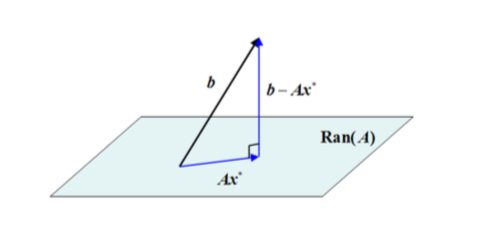
\includegraphics[scale=1]{figuresl/figure2.png}
		\label{default}
	\end{center}
\end{figure}

$\dagger$最小二乘解可能并不唯一, 但分解(15)总是唯一的.
\end{frame}

\begin{frame}
\frametitle{最小二乘与鞍点问题}
线性最小二乘问题 (3.1) 等价于
$$
A^{\top} r=0, \quad r=b-A x
$$
即
\begin{equation}
\left[\begin{array}{cc}{I} & {A} \\ {A^{\top}} & {0}\end{array}\right]\left[\begin{array}{l}{r} \\ {x}\end{array}\right]=\left[\begin{array}{l}{b} \\ {0}\end{array}\right]
\end{equation}
这就是线性最小二乘问题 (3.1) 的\textcolor{blue}{增广方程} (augmented system). 事实上,
方程组 (16) 是下面方程组的一种特殊情形
$$
\left[\begin{array}{cc}{B} & {A} \\ {A^{\top}} & {0}\end{array}\right]\left[\begin{array}{l}{r} \\ {x}\end{array}\right]=\left[\begin{array}{l}{f} \\ {g}\end{array}\right]
$$
其中$B \in \mathbb{R}^{m \times m}$ ~对称半正定. 这就是通常所说的\textcolor{blue}{鞍点问题}. 这个方程组 存在唯一解当且仅当 A 列满秩且矩阵 [B, A] 行满秩.
\end{frame}

\begin{frame}
如果 B 对称正定, 则$r=B^{-1}(f-A x)$,代入第二个方程可得
$$
A^{\top} B^{-1} A x=A^{\top} B^{-1} f-g
$$
这就是\textcolor{blue}{广义的正规方程}. 其所对应的\textcolor{blue}{广义线性最小二乘问题}是
$$
\min _{x \in \mathbb{R}^{n}} \frac{1}{2}\|A x-f\|_{B^{-1}}^{2}+g^{\top} x
$$
其中范数$\|\cdot\|_{B^{-1}}$的定义是$\|x\|_{B^{-1}}^{2}=x^{\top} B^{-1} x$.
\end{frame}

\begin{frame}
\frametitle{5.2 QR分解法}
假定$A \in \mathbb{R}^{m \times n}(m \geq n)$满秩,用三种不同方法来推导

(1)将 Q 的扩充成一个正交矩阵, 记为$[Q, \hat{Q}] \in \mathbb{R}^{m \times m}$于是有
$$	\begin{aligned}\|A x-b\|_{2}^{2} &=\left\|[Q, \hat{Q}]^{\top}(A x-b)\right\|_{2}^{2} \\ &=\left\|[Q, \hat{Q}]^{\top}(Q R x-b)\right\|_{2}^{2} \\ &=\left\|\left[\begin{array}{c}{R x-Q^{\top} b} \\ {-\hat{Q}^{\top} b}\end{array}\right]\right\|_{2}^{2} \\ &=\left\|R x-Q^{\top} b\right\|_{2}^{2}+\left\|\hat{Q}^{\top} b\right\|_{2}^{2} \geq\left\|\hat{Q}^{\top} b\right\|_{2}^{2} \end{aligned}
$$等号成立当且仅当 $R x=Q^{\top} b$所以最小二乘解为
$$
x_{*}=R^{-1} Q^{\top} b
$$
\end{frame}

\begin{frame}
(2)将b写成$b=\left(Q Q^{\top}+I-Q Q^{\top}\right) b$,则
	$$
	\begin{aligned} A x-b &=A x-\left(Q Q^{\top}+I-Q Q^{\top}\right) b \\ &=\left(A x-Q Q^{\top} b\right)-\left(I-Q Q^{\top}\right) b \end{aligned}
	$$
	由于$QQ^{T}$是$Ran(A)$上的正交投影,因此$A x-Q Q^{\top} b$与$\left(I-Q Q^{\top}\right) b$正交. 所以
	$$
	\begin{aligned}\|A x-b\|_{2}^{2} &=\left\|A x-Q Q^{\top} b\right\|_{2}^{2}+\left\|\left(I-Q Q^{\top}\right) b\right\|_{2}^{2} \\ &=\left\|R x-Q^{\top} b\right\|_{2}^{2}+\left\|\left(I-Q Q^{\top}\right) b\right\|_{2}^{2} \\ & \geq\left\|\left(I-Q Q^{\top}\right) b\right\|_{2}^{2} \end{aligned}
	$$等号成立当且仅当$R x=Q^{\top} b$ 所以最小二乘解为
	$$
	x_{*}=R^{-1} Q^{\top} b
	$$
\end{frame}

\begin{frame}
(3)解正规方程. 由定理 5.1 可知, 最小二乘解为
	$$
	\begin{aligned} x_{*} &=\left(A^{\top} A\right)^{-1} A^{\top} b \\ &=\left(R^{\top} Q^{\top} Q R\right)^{-1} R^{\top} Q^{\top} b \\ &=\left(R^{\top} R\right)^{-1} R^{\top} Q^{\top} b \\ &=R^{-1} Q^{\top} b \end{aligned}
	$$
$\dagger$用 QR 分解来求最小二乘解的运算量大约为 $2mn^{2}$ (如果采用 Householder 变换的话, 运算量大约为 $2mn^{2} - 2/3n^{3}$). 当 $m \gg n$ 时, 大约为正规方程的两倍. 当 $m = n$ 时, 几乎相同.\\
$\dagger$通常 QR 算法比较稳定, 是求解最小二乘问题的首选方法, 特别是当 A 条件数较大 (病态) 时.
\end{frame}

\begin{frame}
\frametitle{5.3 奇异值分解法}
设$A \in \mathbb{R}^{m \times n}$列满秩,$A=U\left[\begin{array}{l}{\Sigma} \\ {0}\end{array}\right] V^{\top}$是A的奇异值分解,$U=\left[U_{n}, \tilde{U}\right]$
则
$$
\begin{aligned}\|A x-b\|_{2}^{2}=\left\|U\left[\begin{array}{c}{\Sigma} \\ {0}\end{array}\right] V^{\top} x-b\right\|_{2}^{2} &=\left\|\left[\begin{array}{c}{\Sigma} \\ {0}\end{array}\right] V^{\top} x-\left[U_{n}, \tilde{U}\right]^{\top} b\right\|_{2}^{2} \\ &=\left\|\left[\begin{array}{c}{\Sigma V^{\top} x-U_{n}^{\top} b} \\ {-\tilde{U}^{\top} b}\end{array}\right]\right\|_{2}^{2} \\ &=\left\|\Sigma V^{\top} x-U_{n}^{\top} b\right\|_{2}^{2}+\left\|\tilde{U}^{\top} b\right\|_{2}^{2} \geq\left\|\tilde{U}^{\top} b\right\|_{2}^{2} \end{aligned}
$$
等号当且仅当$\Sigma V^{\top} x-U_{n}^{\top} b=0$时成立, 即
$$
x=\left(\Sigma V^{\top}\right)^{-1} U_{n}^{\top} b=V \Sigma^{-1} U_{n}^{\top} b
$$
这就是线性最小二乘问题 (3.1) 的解.
\end{frame}
\section{广义逆与最小二乘}
\begin{frame}
\frametitle{6 广义逆与最小二乘}
\begin{enumerate}[6.1]
	\item 广义逆的定义
	\item 广义逆的基本性质
	\item 广义逆的计算
    \item 广义逆与线性最小二乘
\end{enumerate}
\end{frame}

\begin{frame}
\frametitle{6.1 广义逆的定义}
\noindent 广义逆的概念最早由 Moore 于 1920 年提出:\\

设$A \in \mathbb{C}^{m \times n}$,若$X \in \mathbb{C}^{n \times m}$满足
\begin{equation}
A X=P_{\operatorname{Ran}(A)}, \quad X A=P_{\operatorname{Ran}(X)}
\end{equation}
即$AX$和$XA$分别为Ran($A$)和Ran($X$)上的正交投影,则称$X$是$A$的
广义逆.
\end{frame}

\begin{frame}
1955 年, Penrose 利用四个矩阵方程给出了广义逆的定义.\\

\textcolor{blue}{定义}~设$A \in \mathbb{C}^{m \times n}$,若$X \in \mathbb{C}^{n \times m}$满足
\begin{equation}
AXA=A 
\end{equation} 
\begin{equation}
XAX=X
\end{equation}
\begin{equation}
(AX)^*=AX
\end{equation}
\begin{equation}
(X A)^{*}=X A 
\end{equation}
则称 X 为 A 的\textcolor{blue}{广义逆} (或 \textcolor{blue}{Moore-Penrose 逆}, 简称 \textcolor{blue}{MP 逆}), 记为 $A\dagger$\\

$\dagger$可以证明, 以上两个定义是等价的.\\

$\dagger$若$A \in \mathbb{C}^{m \times n}$非奇异,则$A^{\dagger}=A^{-1}$
\end{frame}

\begin{frame}
\textcolor{blue}{定理}~设$A \in \mathbb{C}^{m \times n}$则满足矩阵方程 (18)-(21) 的矩阵$X \in \mathbb{C}^{n \times m}$存在唯一,即广义逆存在且惟一.\\

广义逆与SVD\\
设$A \in \mathbb{C}^{m \times n}\operatorname{rank}(A)=r>0, A$的SVD为
$$
A=U\left[\begin{array}{cc}{\Sigma_{1}} & {0} \\ {0} & {0}\end{array}\right] V^{*}, \quad \Sigma_{1}=\operatorname{diag}\left(\sigma_{1}, \sigma_{2}, \ldots, \sigma_{r}\right) \in \mathbb{R}^{r \times r}
$$
则容易验证
$$
A^{\dagger}=V\left[\begin{array}{cc}{\Sigma_{1}^{-1}} & {0} \\ {0} & {0}\end{array}\right] U^{*}
$$
\end{frame}

\begin{frame}
\frametitle{6.2 广义逆的基本性质}
\noindent \textcolor{blue}{定理}~设$A \in \mathbb{C}^{m \times n}$,则\begin{enumerate}[(1)]
	\item $(A^{\dagger})^{\dagger}=A$
	\item $(A^{T})^{\dagger}=(A^{\dagger})^{T},(A^{*})^{\dagger}=(A^{\dagger})^{*}$
	\item $\operatorname{rank}(A)=\operatorname{rank}\left(A^{\dagger}\right)=\operatorname{rank}\left(A^{\dagger} A\right)$
	\item $\left(A A^{*}\right)^{\dagger}=\left(A^{*}\right)^{\dagger} A^{\dagger},\left(A^{*} A\right)^{\dagger}=A^{\dagger}\left(A^{*}\right)^{\dagger}$
	\item $\left(A A^{*}\right)^{\dagger} A A^{*}=A A^{\dagger},\left(A^{*} A\right)^{\dagger} A^{*} A=A^{\dagger} A$
	\item $A^{\dagger}=\left(A^{*} A\right)^{\dagger} A^{*}=A^{*}\left(A A^{*}\right)^{\dagger}$特别地, 若 A 列满秩, 则$A^{\dagger}=\left(A^{*} A\right)^{-1} A^{*}$.若A行满秩,则$A^{\dagger}=A^{*}\left(A A^{*}\right)^{-1}$
	\item 若U,V是酉矩阵,则$(U A V)^{\dagger}=V^{*} A^{\dagger} U^{*}$
\end{enumerate}
\end{frame}

\begin{frame}
$\dagger$一般来说,当A,B是方阵时,
\begin{itemize}
	\item $(A B)^{\dagger} \neq B^{\dagger} A^{\dagger}$
	\item $A A^{\dagger} \neq A^{\dagger} A$
	\item $\left(A^{k}\right)^{\dagger} \neq\left(A^{\dagger}\right)^{k}$
	\item A和$A^{\dagger}$的非零特征值并不是互为倒数
\end{itemize}
设~$A \in \mathbb{C}^{m \times n}$,则
$$
\begin{array}{l}{\operatorname{Ran}\left(A A^{\dagger}\right)=\operatorname{Ran}\left(A A^{*}\right)=\operatorname{Ran}(A)} \\ {\operatorname{Ran}\left(A^{\dagger} A\right)=\operatorname{Ran}\left(A^{*} A\right)=\operatorname{Ran}\left(A^{*}\right)=\operatorname{Ran}\left(A^{\dagger}\right)} \\ {\operatorname{Ker}\left(A A^{\dagger}\right)=\operatorname{Ker}\left(A A^{*}\right)=\operatorname{Ker}\left(A^{*}\right)=\operatorname{Ker}\left(A^{\dagger}\right)} \\ {\operatorname{Ker}\left(A^{\dagger} A\right)=\operatorname{Ker}\left(A^{*} A\right)=\operatorname{Ker}(A)}\end{array}
$$
\end{frame}

\begin{frame}
\frametitle{6.3 广义逆的计算}
\begin{itemize}
	\item \textcolor{blue}{利用SVD},但运算量较大.
	\item \textcolor{blue}{利用满秩分解}\\
	
	\textcolor{blue}{定理}~设$A \in \mathbb{R}^{m \times n}$
	
	(1)若 A 是列满秩矩阵, 则 $A^{\dagger}=\left(A^{*} A\right)^{-1} A^{*}$
	
	(2)若 A 是行满秩矩阵, 则$A^{\dagger}=A^{*}\left(A A^{*}\right)^{-1}$
	
	(3)若A的秩是$r \leq \min \{m, n\}$且其满秩分解为$A=F G$其中$F \in \mathbb{R}^{m \times r}, G \in \mathbb{R}^{r \times n}$,则
		$$
		A^{\dagger}=G^{\dagger} F^{\dagger}=G^{*}\left(G G^{*}\right)^{-1}\left(F^{*} F\right)^{-1} F^{*}
		$$
\end{itemize}
\end{frame}

\begin{frame}
\begin{itemize}
	\item \textcolor{blue}{利用QR分解}\\
	\textcolor{blue}{定理}~设$A \in \mathbb{R}^{m \times n}(m \geq n)$是列满秩矩阵,其QR分解为$A=QR$,其中$Q \in \mathbb{R}^{m \times n}, R \in \mathbb{R}^{n \times n}$,则
	$$
	A^{\dagger}=R^{-1} Q^{*}
	$$
	\item \textcolor{blue}{其他算法}\\
	其他比较重要的算法有: \textcolor{blue}{Greville 递推算法, Cline 算法}等.
\end{itemize}
\end{frame}

\begin{frame}
\frametitle{6.4 广义逆与线性最小二乘}
\noindent \textcolor{blue}{定理}~设$A \in \mathbb{R}^{m \times n}$则线性最小二乘问题的解为
\begin{equation} 
x=A^{\dagger} b+\left(I-P_{A^{\top}}\right) z, \quad \forall z \in \mathbb{R}^{n}
\end{equation}
$\dagger$通常,线性最小二乘问题的解(22)不是唯一的,但当A列满秩时,$P_{A^{\top}}=I$,此时解唯一.\\
\textcolor{blue}{定理}~设$A \in \mathbb{R}^{m \times n}$的解集为$\mathcal{S}$,则
\begin{equation} 
\min _{x \in \mathcal{S}}\|x\|_{2}
\end{equation} 
存在唯一解, 即满足 (23) 的线性最小二乘问题 (3.1) 的解存在且唯一
\end{frame}
\section{最小二乘扰动分析}
\begin{frame}
\frametitle{7 最小二乘扰动分析}
\textcolor{blue}{定理}~设$A \in \mathbb{R}^{m \times n}$且
$\operatorname{rank}(A)=n$设$x$是线性最小二乘问题(3.1)的解,$\tilde{x}$极小化$\|(A+\delta A) \tilde{x}-(b+\delta b)\|_{2}$,则
$$
\frac{\|\tilde{x}-x\|_{2}}{\|x\|_{2}} \leq \varepsilon \cdot\left\{\frac{2 \kappa_{2}(A)}{\cos \theta}+\kappa_{2}^{2}(A) \tan \theta\right\}+O\left(\varepsilon^{2}\right)
$$
其中$\kappa_{2}(A)=\sigma_{1}(A) / \sigma_{n}(A), \theta$为b与$\operatorname{Ran}(A)$的夹角,
$$
\varepsilon \triangleq \max \left\{\frac{\|\delta A\|_{2}}{\|A\|_{2}}, \frac{\|\delta b\|_{2}}{\|b\|_{2}}\right\}
$$
并假定$\varepsilon \cdot \kappa_{2}(A)<1$(确保$A+\delta A$满秩, 从而$\tilde{x}$唯一确定)\\
我们记
$$
\kappa_{L S} \triangleq \frac{2 \kappa_{2}(A)}{\cos \theta}+\kappa_{2}^{2}(A) \tan \theta
$$
\end{frame}

\begin{frame}
这就是最小二乘问题的条件数. 当$\theta=0$,$b \in \operatorname{Ran}(A)$,此时$\kappa_{L S}=2 \kappa_{2}(A)$,当$\theta=\pi / 2$时,$b \perp \operatorname{Ran}(A)$,此时最小二乘解为$x=0$,而$\kappa_{L S}=\infty$;当$0<\theta<\pi / 2$时,$\kappa_{L S}=O\left(\kappa_{2}^{2}(A)\right)$

定义残量$r=b-A x, \tilde{r}=(b+\delta b)-(A+\delta A) \tilde{x}$,我们有下面的性质 \textcolor{blue}{[Higham2002]}
$$
\frac{\|\tilde{r}-r\|_{2}}{\|r\|_{2}} \leq 1+2 \varepsilon \cdot \kappa_{2}(A)
$$
当我们使用 QR 分解或 SVD 分解求解最小二乘问题时, 由于采用的是正 交变换, 它们都是数值稳定的. 而正规方程涉及求解方程组
$A^{\top} A x=A^{\top} b$,其精度依赖于条件数$\kappa_{2}\left(A^{\top} A\right)=\kappa_{2}^{2}(A)$,因为其误差是以$\kappa_{2}^{2}(A)$倍数增长. 因此当 A 的条件数较大时, 正规方程法的精度会大大降低.
\end{frame}
\section{最小二乘问题的推广及其应用}
\begin{frame}
\frametitle{8 最小二乘问题的推广及其应用}
\begin{enumerate}[8.1]
	\item 正规法
	\item 加权正则化
	\item 约束最小二乘问题
	\item 应用:多项式数据拟合
	\item 应用:线性预测
	\item 应用:信号处理
\end{enumerate}
\end{frame}

\begin{frame}
\frametitle{8.1 正则化}
在求解超定线性方程组时, 我们极小化$\|A x-b\|_{2}^{2}$而对于欠定线性方程组, 我们极小化的是$\|x\|_{2}^{2}$.两者合起来就是
\begin{equation}
\min _{x \in \mathbb{R}^{n} \times n} \frac{1}{2}\|A x-b\|_{2}^{2}+\frac{\alpha}{2}\|x\|_{2}^{2}
\end{equation}
其中$\alpha>0$是权系数. 对应的目标函数记为
$$
J(x)=\|A x-b\|_{2}^{2}+\alpha\|x\|_{2}^{2}
$$
当$\alpha>0$时,$J(x)$是一个严格凸的二次函数, 因此存在唯一的最小值点.关于 $x$ 求导后, 令其等于零, 可得
$$
\left(A^{\top} A+\alpha I\right) x=A^{\top} b
$$
由于$A^{\top} A+\alpha I$对称正定, 故非奇异. 所以问题 (24) 的唯一解为
$$
x=\left(A^{\top} A+\alpha I\right)^{-1} A^{T} b
$$
\end{frame}

\begin{frame}
\frametitle{8.2 加权正则化}
一类应用更广泛的问题是下面的加权正则化问题
\begin{equation}
\min _{x \in \mathbb{R}^{n} \times n} \frac{1}{2}\|A x-b\|_{2}^{2}+\frac{\alpha}{2}\|W x\|_{2}^{2}
\end{equation}
其中$W \in \mathbb{R}^{p \times n}$是广义加权矩阵, 可以是非负对角矩阵, 对称正定矩阵, 也可以是一般矩阵 (如一阶差分算子, 二阶差分算子等). 注意, W 不一定 要求是方阵.\\
经过类似的推导,问题(25) 的解满足
$$
\left(A^{\top} A+\alpha W^{\top} W\right) x=A^{\top} b
$$
如果$A^{\top} A+\alpha W^{\top} W$非奇异, 则存在唯一解
$$
x=\left(A^{\top} A+\alpha W^{\top} W\right)^{-1} A^{T} b
$$
\end{frame}

\begin{frame}
\frametitle{8.3 约束最小二乘问题}
考虑带有约束的最小二乘问题
\begin{equation}
\begin{array}{l}{\min _{x \in \mathbb{R}^{n \times n}} \frac{1}{2}\|A x-b\|_{2}^{2}} \\ {\text { s.t. } \quad B x=f}\end{array}
\end{equation}
其中$B x=f$是约束条件. 对应的 Lagrange 函数为
$$
J(x)=\frac{1}{2}\|A x-b\|_{2}^{2}+\lambda^{\top}(B x-f)
$$
分别对 $x$ 和 $\lambda$ 求一阶导数, 并令其等于零, 可得
$$
\left[\begin{array}{cc}{A^{\top} A} & {B^{\top}} \\ {B} & {0}\end{array}\right]\left[\begin{array}{l}{x} \\ {\lambda}\end{array}\right]=\left[\begin{array}{c}{A^{\top} b} \\ {f}\end{array}\right]
$$
\end{frame}

\begin{frame}
如果$A^{\top} A$非奇异, 且 B 行满秩, 则存在唯一解
$$
\begin{array}{l}{\lambda=\left[B\left(A^{\top} A\right)^{-1} B^{\top}\right]^{-1}\left[B\left(A^{\top} A\right)^{-1} A^{\top} b-f\right]} \\ {x=\left(A^{\top} A\right)^{-1}\left(A^{\top} b-B^{\top} \lambda\right)}\end{array}
$$
\end{frame}

\begin{frame}
\frametitle{8.4 应用: 多项式数据拟合}
\noindent 已知n个点$\left\{\left(t_{i}, f_{i}\right)\right\}_{i=1}^{n}$,寻找一个低次多项式来拟合这些数据. 设拟合多项式为
$$
p(x)=a_{0}+a_{1} t+a_{2} t^{2}+\cdots+a_{m} t^{m}
$$
通常$m \ll n$将上述n个点代入可得
$$
\left[\begin{array}{ccccc}
{1} & {t_{1}} & {t_{1}^{2}} & {\cdots} & {t_{1}^{m}} \\
{1} & {t_{2}} & {t_{2}^{2}} & {\cdots} & {t_{2}^{m}} \\ {\vdots} & {\vdots} & {\vdots} & {} & {\vdots} \\
{1} & {t_{n}} & {t_{n}^{2}} & {\cdots} & {t_{n}^{m}}\end{array}\right]_{n \times(m+1)}\left[\begin{array}{c}{a_{0}} \\ 
{a_{1}} \\ 
{\vdots} \\ 
{a_{m}}
\end{array}\right]=\left[\begin{array}{c}{f_{1}} \\ {f_{2}} \\ {\vdots} \\ {f_{n}}\end{array}\right] or ~~A x=f
$$
其中$A \in \mathbb{R}^{n \times(m+1)}, x=\left[a_{0}, a_{1}, \ldots, a_{m}\right]^{\top}$,由于$m \ll n$该方程组是超定 的, 解通常是不存在的. 因此, 我们寻找一个近似解, 使得残量
$\|f-A x\|_{2}$最小, 即求解最小二乘问题
$$
\min _{x \in \mathbb{R}^{m+1}}\|f-A x\|_{2}^{2}
$$
\end{frame}

\begin{frame}
\frametitle{8.5 应用: 线性预测}
预测一个时间序列的未来走向, 一个常用方法就是线性预测. 假定在 $t_{k}$ 时刻的值 $f_{k}$ 线性依赖于其前 m 个时刻的值$f_{k-1}, f_{k-2}, \dots, f_{k-m}$,即
\begin{equation}
f_{k}=a_{1} f_{k-1}+a_{2} f_{k-2}+\cdots+a_{m} f_{k-m}
\end{equation}
现在已经测得该时间序列的前 n 个值$f_{i}, i=0,1,2, \ldots, n-1$,其中$n \gg m$.\textcolor{blue}{如何预测其未来的取值?}
将现有的数据代入上述关系式可得
$$
\left[\begin{array}{ccccc}
{f_{m-1}} & {f_{m-2}} & {f_{m-3}} & {\cdots} & {f_{0}} \\
{f_{m}} & {f_{m-1}} & {f_{m-2}} & {\cdots} & {f_{1}} \\ 
{\vdots} & {\vdots} & {\vdots} & {} & {\vdots} \\ 
{f_{n-2}} & {f_{n-3}} & {f_{n-4}} & {\cdots} & {f_{n-m-1}}
\end{array}\right]_{(n-m) \times m}\left[\begin{array}{c}
{a_{1}} \\
{a_{2}} \\
{\vdots} \\ 
{a_{m}}
\end{array}\right]=\left[\begin{array}{c}
{f_{m}} \\ 
{f_{m+1}} \\ 
{\vdots} \\ 
{f_{n-1}}
\end{array}\right]或A x=f
$$
这也是一个超定问题, 因此需要求解最小二乘$\min _{x \in \mathbb{R}^{m}}\|f-A x\|_{2}^{2}$
\end{frame}

\begin{frame}
\frametitle{8.6 应用: 信号处理}
\begin{itemize}
	\item 信号去噪 : 在获取数字信号时, 由于各种各样的原因, 最后得到的信 号总会带有一定的噪声. 去噪是数字信号和图像处理中的一个基本 问题. 其中一个有效方法就是加权最小二乘法.
	$$
	\min _{x} \frac{1}{2}\|x-b\|_{2}^{2}+\frac{1}{2} \alpha\|D x\|_{2}^{2}
	$$
	其中 D 是离散的二阶导算子.
\end{itemize}
	\begin{figure}[htbp]
		\begin{center}
			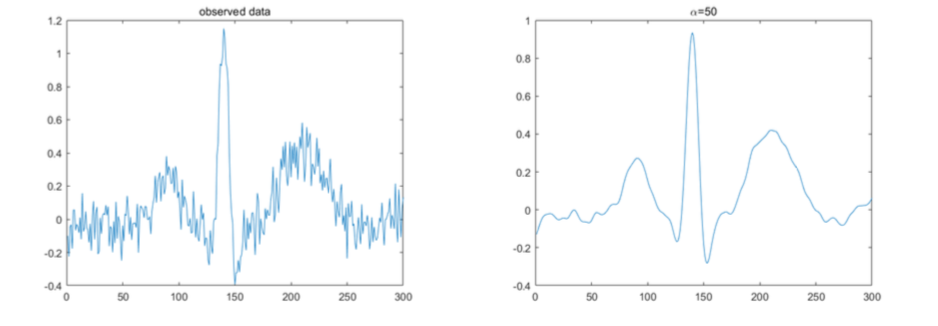
\includegraphics[scale=0.5]{figuresl/figure3.png}
		\end{center}
	\end{figure}
\end{frame}

\begin{frame}
\begin{itemize}
	\item 图像去模糊\\
	一般模型:
	$$
	f=K(x)+n
	$$
	其中 x 表示真实图像, f 表示观察到的图像,$K(\cdot)$是一个卷积算子, 代表模糊机制, n 代表噪声.
	\item 图像压缩
\end{itemize}
\end{frame}


\end{document}
